\documentclass[twocolumn, 9pt]{article}

\usepackage{times}

\usepackage[T1]{fontenc}
\usepackage[explicit]{titlesec}
\usepackage[font=small,labelfont=bf]{caption}
\usepackage[toc,page]{appendix}
\usepackage{algpseudocode}
\usepackage{amsmath}
\usepackage{amssymb}
\usepackage{balance}
\usepackage{booktabs} % For formal tables
\usepackage{enumitem}
\usepackage{hyperref}
\usepackage{listings}
\usepackage{microtype}
\usepackage{multirow}
\usepackage{siunitx}
\usepackage{subcaption}
\usepackage{tikz}
\usepackage{varwidth}
\usepackage{xcolor}

\hypersetup{
  colorlinks=true,
  linkcolor=ACMRed,
  urlcolor=ACMBlue,
  citecolor=ACMRed,
}

\lstset{
  captionpos=b,
  showspaces=false,
  showtabs=false,
  breaklines=true,
  showstringspaces=false,
  breakatwhitespace=true,
  escapeinside={(*@}{@*)},
  basicstyle=\footnotesize\ttfamily,
  columns=fullflexible,
  morekeywords={maybe_downsample, maybe_skip, maybe}
}

\captionsetup[lstlisting]{font={footnotesize}}
\renewcommand{\lstlistingname}{Example}

% \makeatletter
% \newcommand\appendix@section[1]{%
%   \refstepcounter{section}%
%   \orig@section*{Appendix \@Alph\c@section: #1}%
%   \addcontentsline{toc}{section}{Appendix \@Alph\c@section: #1}%
% }
% \let\orig@section\section
% \g@addto@macro\appendix{\let\section\appendix@section}
% \makeatother

% \newcommand*{\Appendixautorefname}{Appendix}

\frenchspacing

%%%%%%%%%%%%%%%%%%%%%%%%%%%%%%%%%%%%%%%%%%%%%%%%%%%%%%%%%%%%%%%
%% Paper setup
%%%%%%%%%%%%%%%%%%%%%%%%%%%%%%%%%%%%%%%%%%%%%%%%%%%%%%%%%%%%%%%

\newcommand{\sysname}{AWStream}
\newcommand{\para}[1]{\smallskip\noindent\textbf{#1}}
\newcommand{\paraf}[1]{\noindent\textbf{#1}}
\newcommand{\todo}[1]{{\color{ACMRed}\bf{TODO: #1}\normalfont}}
\newcommand{\fixme}[1]{{\color{ACMRed}\bf{FIXME: #1}\normalfont}}
\newcommand{\question}[1]{{\color{ACMRed}\footnotesize{Q: #1}\normalfont}}

\newcommand{\maybe}{\texttt{maybe}}

\def\Snospace~{\S{}}
\renewcommand*\sectionautorefname{\Snospace}
\renewcommand*\subsectionautorefname{\Snospace}
\renewcommand*\subsubsectionautorefname{\Snospace}
\renewcommand*{\equationautorefname}{Eq.}
\renewcommand*{\figureautorefname}{Fig.}

\newcommand{\specialcell}[2][c]{%
  \begin{tabular}[#1]{@{}c@{}}#2\end{tabular}}

\newcommand*\circled[1]{\tikz[baseline=(char.base)]{
    \node[shape=circle,draw,inner sep=0.5pt] (char) {#1};}}

\newcommand*\qe{$\text{Q}_\text{E}$}
\newcommand*\qc{$\text{Q}_\text{C}$}
\newcommand*\rc{$\text{R}_\text{C}$}
\newcommand*\spd{$\text{S}_\text{ProbeDone}$}

%%% Local Variables:
%%% mode: latex
%%% TeX-master: "awstream"
%%% End:

\begin{document}
\title{\sysname{}: Adaptive Wide-Area Streaming Analytics \\ Appendix}
\author{ \textit{Paper \#8} }
\date{}
\maketitle

\section{WAN Bandwidth Characteristics}

\autoref{fig:aws-bandwidth} shows the available bandwidth between Amazon EC2
servers (Tokyo, Ireland, N. Virginia, N. California) in our day-long
measurements. Most inter-continental links (between Ireland and all others,
between Tokyo and N. Virginia) have limited bandwidth (\textasciitilde 50
mbps). Other pairs exhibit large variations from 10 mbps up to 150 mbps.

\begin{figure}
  \centering
  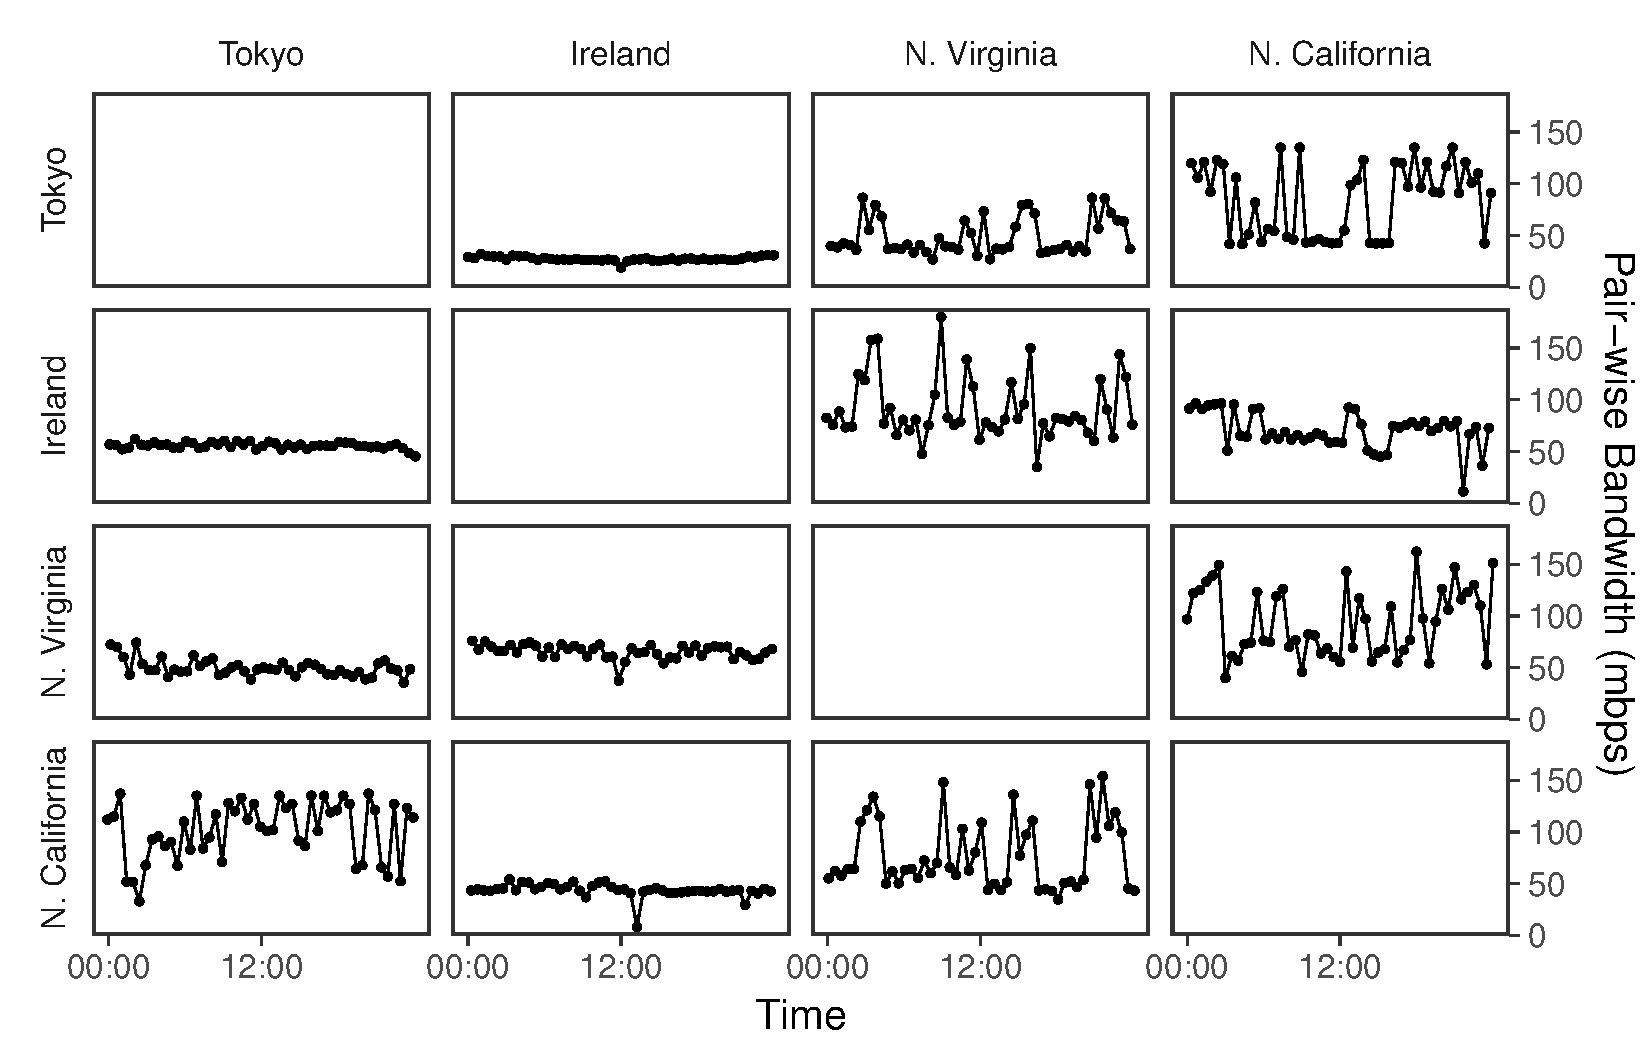
\includegraphics[width=1\columnwidth]{figures/aws-bandwidth.pdf}
  \caption{Pair-wise bandwidth in time series from our day-long measurements.}
  \label{fig:aws-bandwidth}
\end{figure}

\section{Application Implementations}
\label{appendix:appl-impl}

Below we provide details about how we implement our three applications
(\autoref{fig:three-apps}), including the libraries we use and how we integrate
them into \sysname{}.

\para{Augmented Reality.} We target at mobile augmented reality applications
that recognize objects by offloading the heavy computation to resources
elsewhere, e.g.\,the cloud.  Image-related operations use OpenCV
3.1~\cite{opencvlibrary} and object recognition uses YOLO~\cite{darknet13,
  redmon2016yolo9000}, a GPU-enabled pre-trained neural network. Videos are
encoded with H.264~\cite{richardson2011h} because of its prevalence in existing
systems. Our implementation uses GStreamer~\cite{gstreamer} with
\texttt{x264enc} plugin. To integrate with \sysname{}, we first create a
pipeline that exposes \texttt{appsrc} (to feed raw image data) and
\texttt{appsink} (to get encoded bytes). The GStreamer main loop executes in a
separate thread and \sysname{} communicates with it via Rust's channel. The
\texttt{x264enc} uses the \texttt{zerolatency} preset and four threads. We use
constant quality encoding and expose the quantization factor as a knob (in
addition to image resolutions and frame rates).

Object recognition returns a list of bounding boxes with the type of the object,
and each bounding box is a rectangle with normalized coordinates on the
image. We compare the detection against the reference result from raw data, and
declare it success if the intersection over union (IOU) is greater than
50\%~\cite{everingham2010pascal} and the object type matches. We use F1
score~\cite{Rijsbergen:1979:IR:539927} as the accuracy function. In terms of
dataset, we collected our own video clips: the training data is a 24-second long
video of an office environment; the test data is a 246-second long video of a
home environment.

\para{Pedestrian Detection.} This application analyzes streams of videos from
installed CCTV cameras and detects pedestrians inside. We use a similar setup
(OpenCV and GStreamer) as our augmented reality application except for the
analytical function. To detect pedestrians, we use histogram of oriented
gradients (HOG)~\cite{dalal2005histograms} with the default linear SVM
classifier from OpenCV. To ensure real-time processing of frames,
GPU-accelerated implementation is used. Because we do not recognize individual
pedestrians, a successful detection in this case only requires matching the
bounding box. Our evaluation uses MOT16 dataset~\cite{milan2016mot16} for both
profiling and runtime.

\begin{figure}
  \centering
  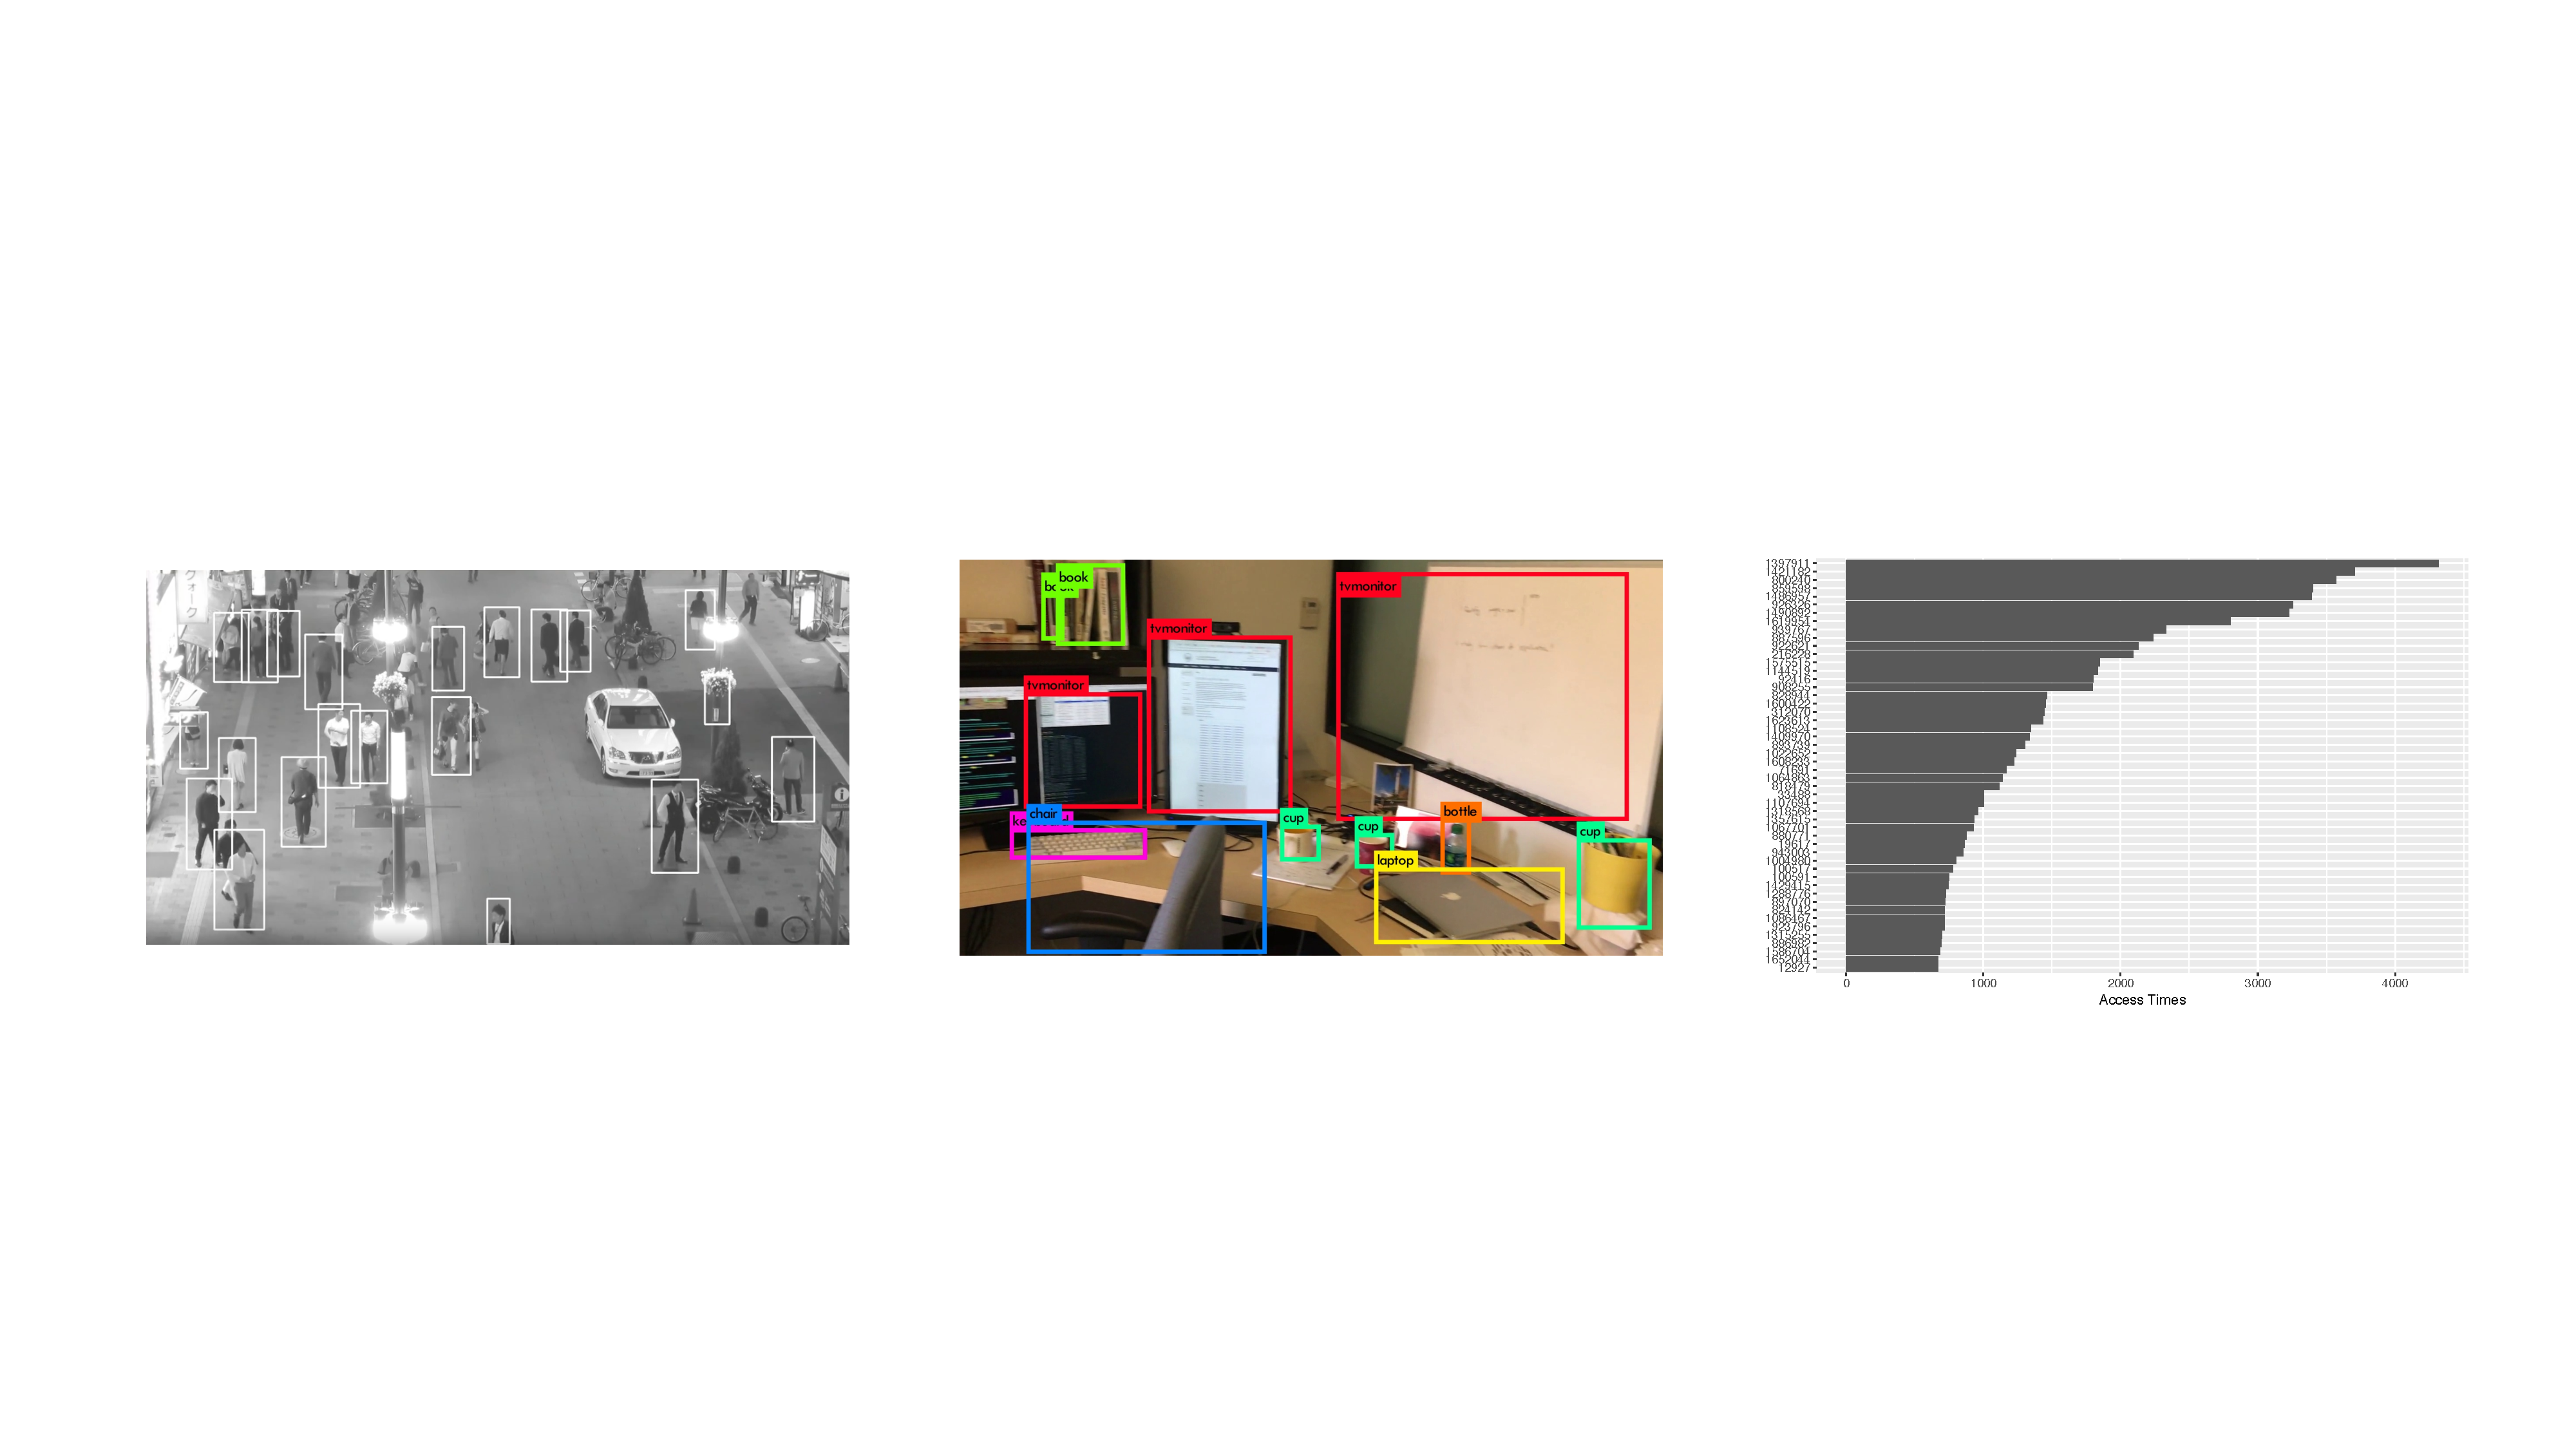
\includegraphics[width=\columnwidth]{figures/apps.pdf}
  \caption{Three applications: augmented reality, pedestrian detection, and
    distributed Top-K.}
  \label{fig:three-apps}
\end{figure}

\begin{figure}
  \centering
  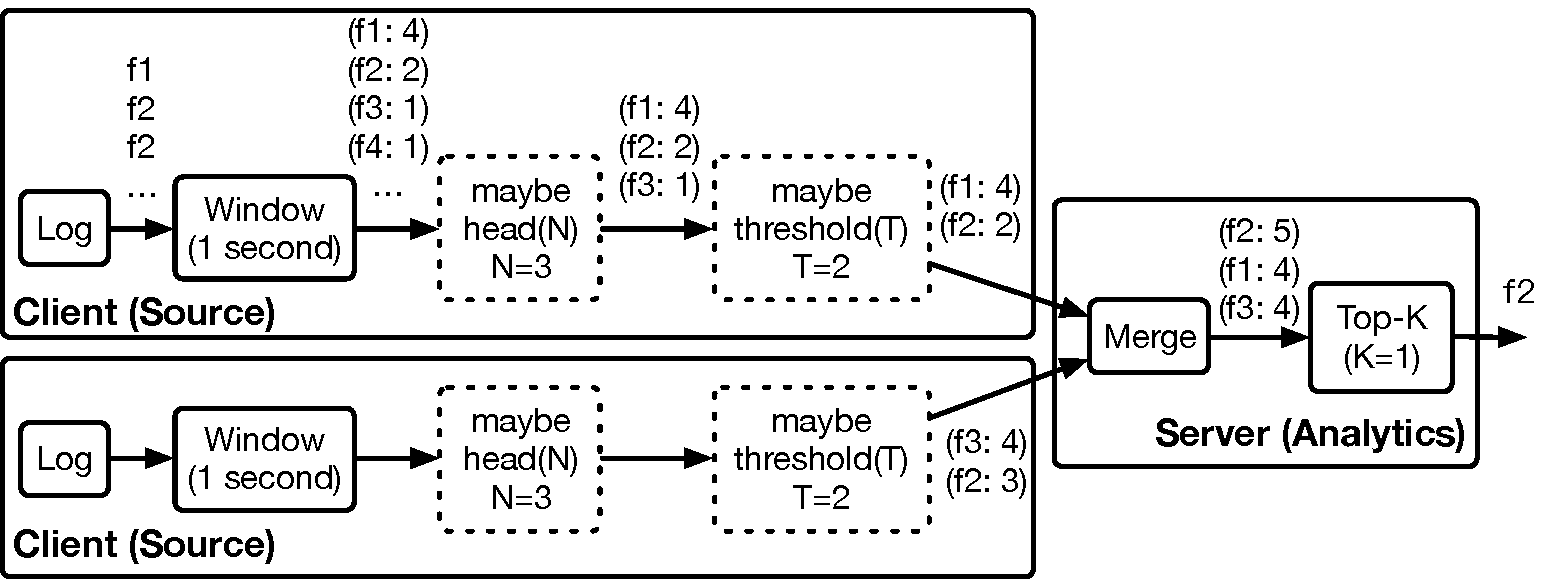
\includegraphics[width=\columnwidth]{figures/topk.pdf}
  \caption{A distributed Top-K application with two degradation operations:
    \texttt{head} and \texttt{threshold}. Discarding data with these two
    operations will affect final results. In this example, \texttt{f2}, which is
    not in Top-1 for either client, becomes the global Top-1 after the merge. It
    would have been purged if the clients use threshold T=3.}
  \label{fig:topk}
\end{figure}

\para{Distributed Top-K.} Many monitoring applications need to answer the
\textit{Top-K} question~\cite{babcock2003distributed}, such as the Top-K most
popular URLs, or the Top-K most access files. A distributed Top-K application
aggregates information from geo-distributed servers to computer a final Top-K.

\autoref{fig:topk} shows the Top-K processing pipeline with example data. Source
nodes first performs a \texttt{Window} operation to generate data summary, which
is key-value pairs \texttt{(item: count)} for each item. After the summary, the
data size can still be too large because most real-world access patterns follow
a long tail distribution: there is a large-but-irrelevant tail that contributes
little to Top-K. The source nodes perform two degradation operations: (1) a
head(\texttt{N}) operation that only takes the top \texttt{N} entries; (2) a
threshold(\texttt{T}) that filters small entries whose count is smaller than
\texttt{T}. These two operations are not orthogonal. Their impact on data size
reduction and quality degradation depends on the data distribution.

For accuracy, we use Kendall's~$\tau$~\cite{abdi2007kendall}, a correlation
measure of the concordance between two ranked list. The output ranges from
\(-1\) to 1, representing no agreement to complete agreement. To integrate with
\sysname{}, we convert Kendall's~$\tau$ to the range of [0, 1] with a linear
transformation.

Our Top-K application aims to find the Top-50 most accessed files from web
server logs. We use Apache log files that record and store user access
statistics for the \href{https://www.sec.gov}{SEC.gov} website. The logs are
split into four groups, simulating four geo-distributed nodes monitoring web
accesses. To match the load of popular web servers, we compress one hour's logs
into one second.

\section{JetStream++}
\label{appendix:jetstream++}

We modified the open source version of
JetStream\footnote{\url{https://github.com/princeton-sns/jetstream/}, commit
  bf0931b2d74d20fdf891669188feb84c96AF84.} in order to use our profile as its
manual policy. Because JetStream doesn't support simultaneous degradation across
multiple operators, we implemented a simple \texttt{VideoSource} operator that
understands how to change image resolutions, frame rate, and video encoding
quantization. At runtime, \texttt{VideoSource} queries congestion policy manager
and adjusts three dimensions simultaneously. This operator is then exposed to
the Python-implemented control plane. We call this modified version
JetStream++.\footnote{URL to our patch is elided for anonymity.}

%% https://github.com/nebgnahz/jetstream-clone/pull/2/files}

JetStream's code base is modular and extensible: the modifications include 53
lines for the header file, 171 lines for implementation, 75 lines for unit test,
and 49 lines of python as the application. While extending JetStream with our
profile is not challenging, JetStream++ performs degradation in a single
operator and loses the composability. We could modify JetStream to support
degradation across multiple operators, but that would require substantial
changes to JetStream. Using JetStream++ with our profile, the comparison is
enough to illustrate the difference between \sysname{}'s and JetStream's
runtime.

\section{Runtime Evaluation of PD and TK}
\label{appendix:more-runtime}

 % > summary(latency)
 %      Time        JetStream++        JetStream            HLS
 % Min.   :206.0   Min.   :  46.68   Min.   :   82.4   Min.   :1887
 % 1st Qu.:264.2   1st Qu.: 380.70   1st Qu.: 1435.7   1st Qu.:2320
 % Median :322.5   Median : 597.67   Median : 1534.9   Median :2623
 % Mean   :322.5   Mean   : 624.21   Mean   : 2629.2   Mean   :2610
 % 3rd Qu.:380.8   3rd Qu.: 831.75   3rd Qu.: 1688.1   3rd Qu.:2863
 % Max.   :439.0   Max.   :1388.79   Max.   :11489.3   Max.   :4227
 % NA's   :1       NA's   :1         NA's   :1         NA's   :1
 %
 % Streaming over TCP Streaming over UDP    AWStream
 % Min.   :   878.8   Min.   :29.70      Min.   : 48.35
 % 1st Qu.: 26176.3   1st Qu.:31.18      1st Qu.: 63.58
 % Median : 50679.0   Median :32.68      Median : 77.98
 % Mean   : 52130.4   Mean   :32.89      Mean   :105.56
 % 3rd Qu.: 76010.8   3rd Qu.:34.60      3rd Qu.:124.71
 % Max.   :111455.7   Max.   :36.30      Max.   :417.79
 % NA's   :1          NA's   :1          NA's   :1
 %%
 %% 20x over JetStream, 7.7x over JetStream++

 % > summary(accuracy)
 %      Time        JetStream++       JetStream           HLS
 % Min.   :206.0   Min.   :0.6735   Min.   :0.7822   Min.   :0.00000
 % 1st Qu.:264.2   1st Qu.:0.7871   1st Qu.:0.8247   1st Qu.:0.04077
 % Median :322.5   Median :0.8285   Median :0.8420   Median :0.06372
 % Mean   :322.5   Mean   :0.8232   Mean   :0.8395   Mean   :0.09429
 % 3rd Qu.:380.8   3rd Qu.:0.8667   3rd Qu.:0.8531   3rd Qu.:0.09346
 % Max.   :439.0   Max.   :0.9148   Max.   :0.9130   Max.   :0.69602
 % NA's   :1       NA's   :1        NA's   :1        NA's   :1
 % Streaming over TCP Streaming over UDP      AWStream
 % Min.   :0.8502     Min.   :-0.0000985   Min.   :0.7899
 % 1st Qu.:0.9012     1st Qu.: 0.0021567   1st Qu.:0.8405
 % Median :0.9150     Median : 0.0068409   Median :0.8552
 % Mean   :0.9150     Mean   : 0.0314461   Mean   :0.8622
 % 3rd Qu.:0.9295     3rd Qu.: 0.0312727   3rd Qu.:0.8805
 % Max.   :0.9697     Max.   : 0.6220806   Max.   :0.9853
 % NA's   :1          NA's   :1            NA's   :1
 %%
 %% 6% drop

In the main paper, we presented the evaluation results for AR. Now we show the
relevant details and results for the remaining two applications: PD and TK.

\paraf{Pedestrian Detection.} The setup for PD is the same with AR: three Amazon
EC2 as clients and one as server. The maximal configuration $c_{\max}$ is
1920x1080 resolution, \(10~\text{FPS}\) and a quantization of 20; it consumes
about 12 mbps. For PD, \sysname{} learns that frame rate is less important than
resolution. It favors 10FPS with 1080p instead of 30FPS with 900p as in AR.

When running experiments, we use the same bandwidth shaping schedule as we used
for AR. Baselines are also the same: Streaming over TCP, streaming over UDP,
JetStream, JetStream++, and HLS.

\begin{figure}[t]
  \begin{subfigure}[t]{\columnwidth}
    \centering
    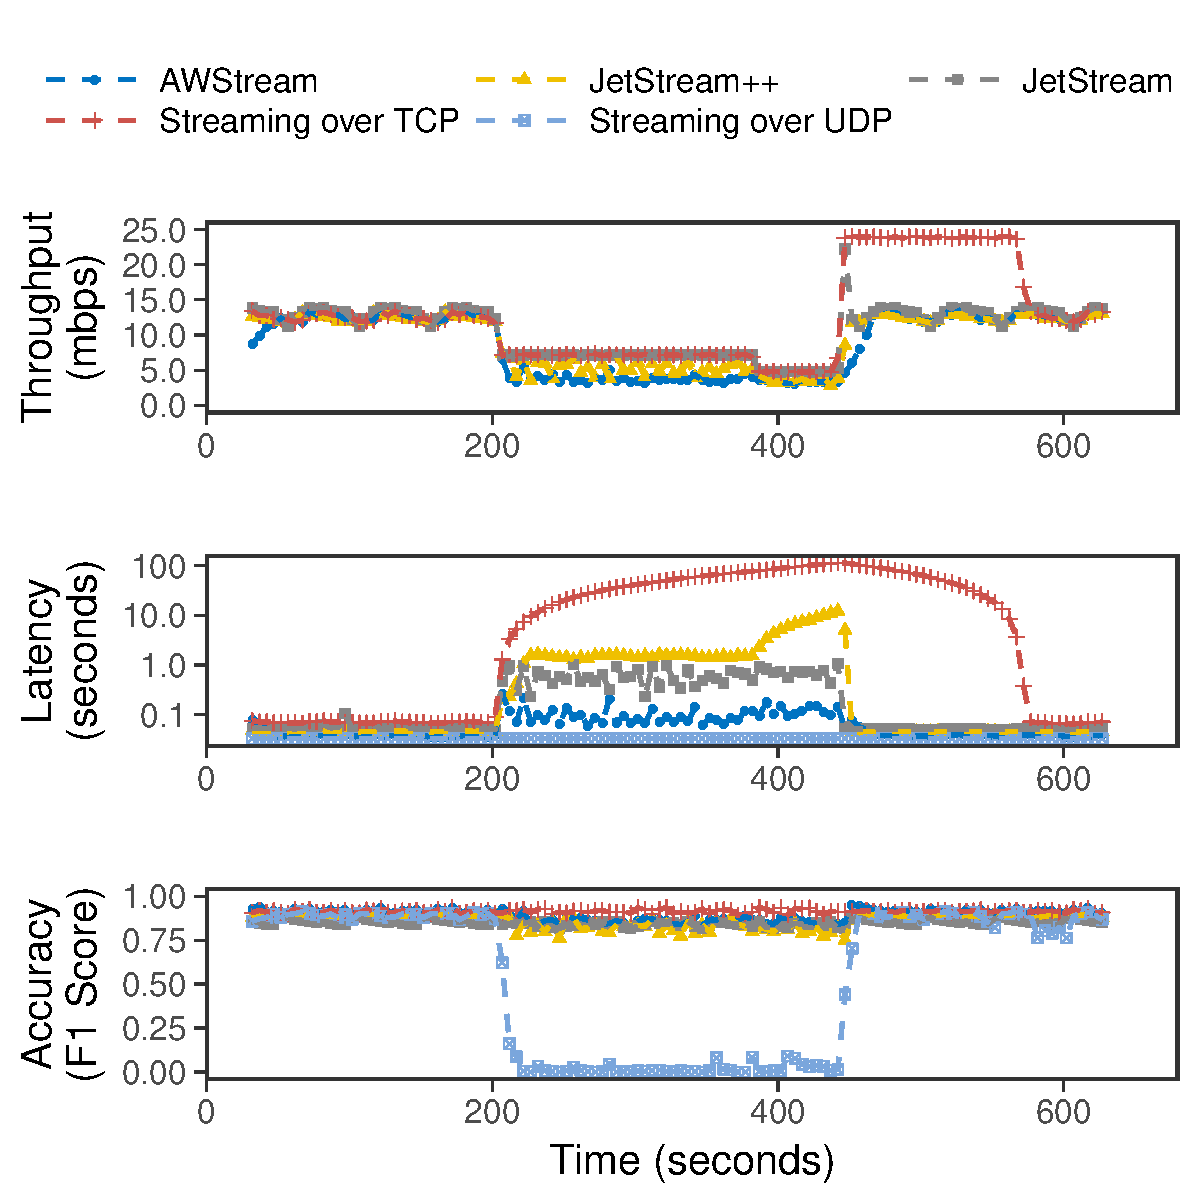
\includegraphics[width=\columnwidth]{figures/runtime_mot-timeseries.pdf}
    \caption{PD's runtime behavior with a time-series plot: throughput (top),
      showing the effect of bandwidth shaping; latency (middle) in log scale;
      and accuracy (bottom).}
    \label{fig:pd-runtime-timeseries}
  \end{subfigure}
  \vspace{1em}
  \\
  \begin{subfigure}[t]{\columnwidth}
    \centering
    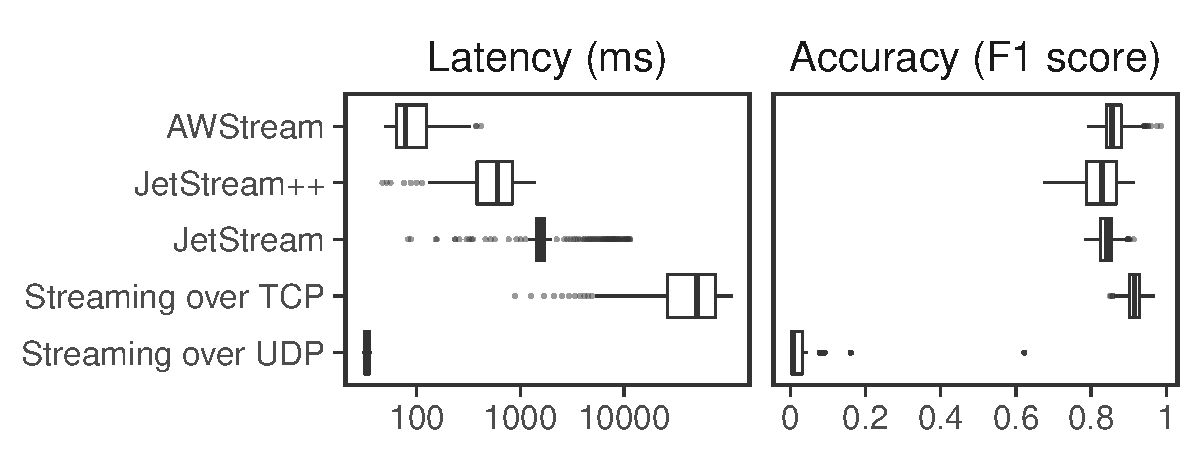
\includegraphics[width=\columnwidth]{figures/runtime_mot-boxplot.pdf}
    \caption{PD's performance summary of latency and accuracy during the traffic
      shaping (between t=200s and t=440s).}
    \label{fig:pd-runtime-boxplot}
  \end{subfigure}
  \caption{PD runtime evaluation.}
  \label{fig:pd-runtime}
\end{figure}

\begin{figure}[t]
  \begin{subfigure}[t]{\columnwidth}
    \centering
    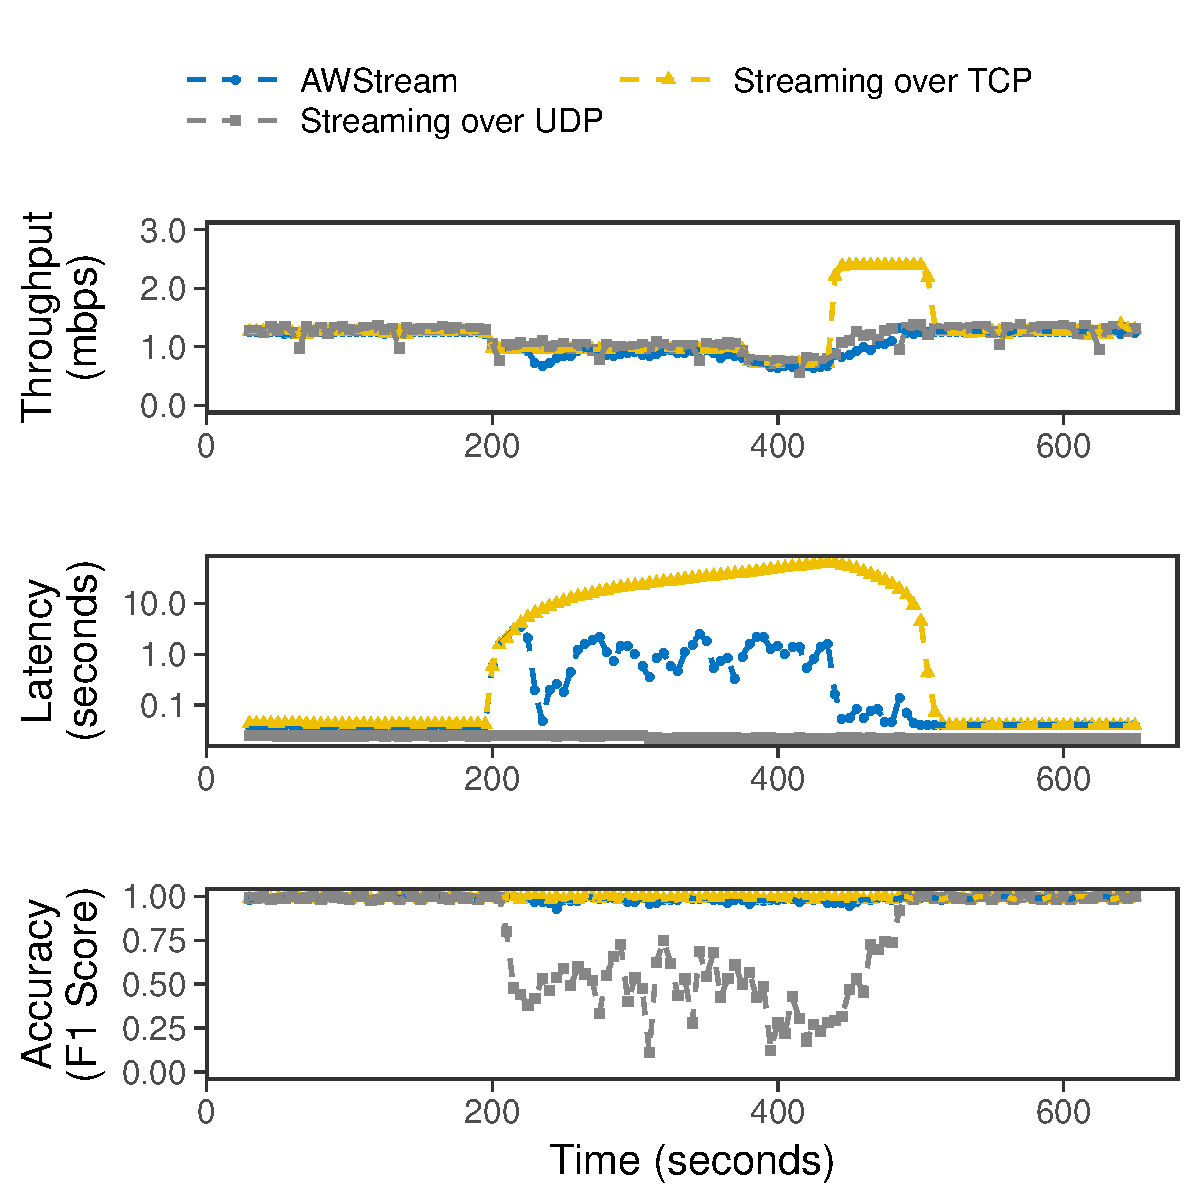
\includegraphics[width=\columnwidth]{figures/runtime_tk-timeseries.pdf}
    \caption{TK's runtime behavior with a time-series plot: throughput (top),
      showing the effect of bandwidth shaping; latency (middle) in log scale;
      and accuracy (bottom).}
    \label{fig:tk-runtime-timeseries}
  \end{subfigure}
  \vspace{1em}
  \\
  \begin{subfigure}[t]{\columnwidth}
    \centering
    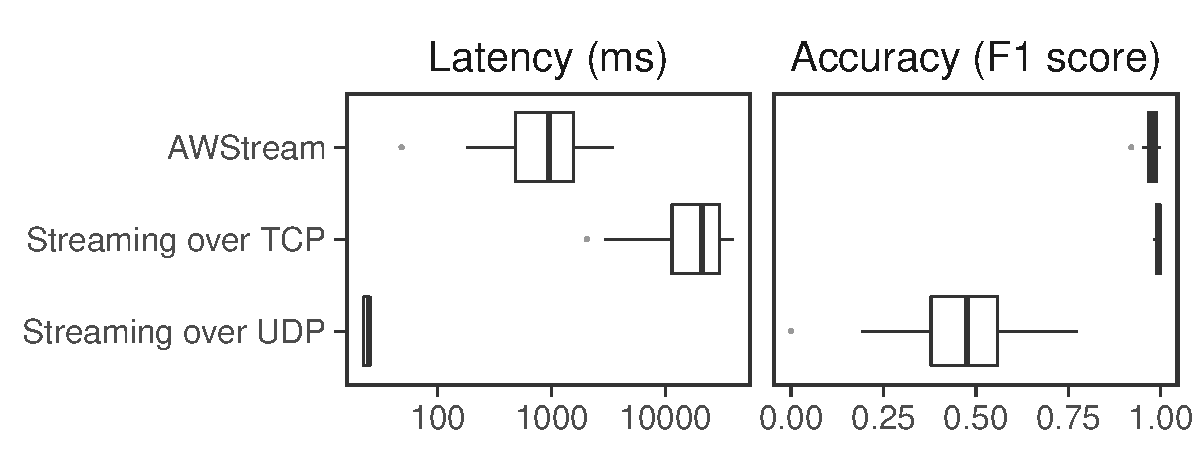
\includegraphics[width=\columnwidth]{figures/runtime_tk-boxplot.pdf}
    \caption{TK's performance summary of latency and accuracy during the traffic
      shaping (between t=200s and t=440s).}
    \label{fig:tk-runtime-boxplot}
  \end{subfigure}
  \caption{TK runtime evaluation.}
  \label{fig:tk-runtime}
\end{figure}


\autoref{fig:pd-runtime} shows the runtime behavior in both time series
(throughout the experiment) and box plot (between t=200s and t=440s).  Most
observations we made in the main paper are the same here: $(i)$~Streaming with
TCP has the highest accuracy (median 92\%) at a cost of high
latency. $(ii)$~Streaming with UDP has the lowest bounded latency but the
accuracy is too low. $(iii)$~HLS incurs a latency of 2-3 seconds due to
chunking, buffering, and client fetching; its accuracy in PD is quite poor
because HLS reduces latency and encoding quality. $(iv)$~JetStream and
JetStream++ can balance latency and accuracy; but JetStream's manual policy is
unable to sustain 5mps bandwidth, so its median latency is high (1535ms);
JetStream++'s latency is lower (598ms) than JetStream, but its accuracy (82\%)
suffers from policy oscillation. \sysname{} is able to achieve the lowest
latency (78ms) with small accuracy drop (86\%, 6\% drop in comparison to
TCP). In comparison to the state-of-the-art system JetStream, \sysname{}
improves the latency by 20$\times$ (from 1535ms to 78ms) and accuracy by 1\%
(from 84\% to 85\%).

\begin{figure*}[t]
  \centering
  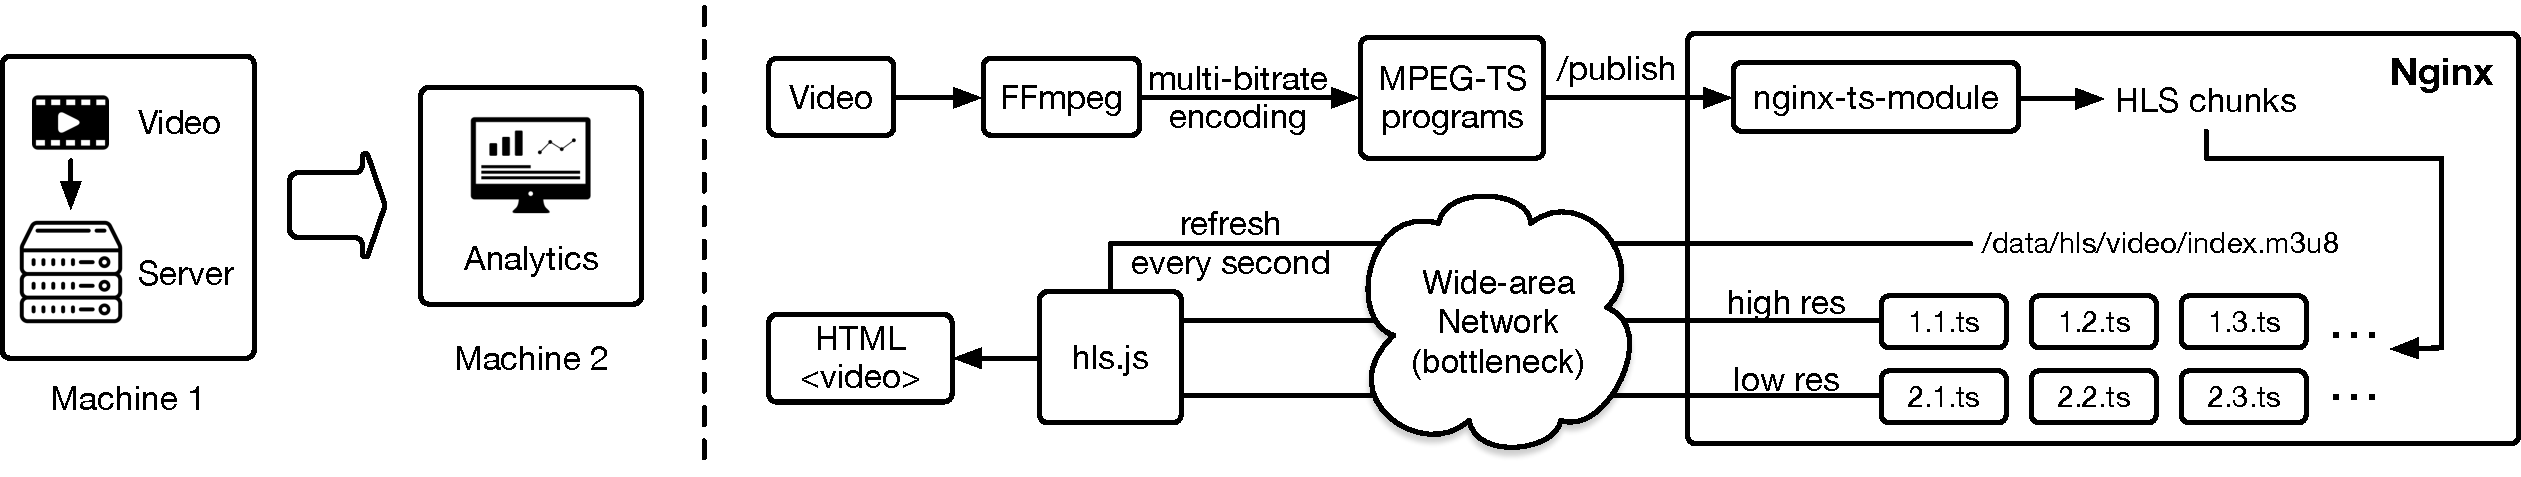
\includegraphics[width=\textwidth]{figures/hls-arch.pdf}
  \caption{HLS setup. (Left) High-level overview: machine 1 generates a video
    and stores it in the server; machine 2 fetches the data and performs
    analytics. (Right) Detailed view: (1)~FFmpeg encodes video with multiple
    bitrates and groups them into MPEG-TS programs; (2)~\texttt{nginx-ts-module}
    then generates HLS chunks on the fly and stores them for nginx serving;
    (3)~the client (using \texttt{hls.js}) periodically fetches the latest index
    file (\texttt{index.m3u8}) and then downloads the right chunk according to
    network conditions.}
  \label{fig:hls-arch}
\end{figure*}

\para{Top-K.} For TK, our logs are split into four groups. We then use four
Amazon EC2 as clients and one as server. The maximal configuration $c_{\max}$ is
$N=9750$ for \texttt{head} and $T=0$ for \texttt{threshold}; it consumes about
1.2 mbps. Because the overall bandwidth consumption is much smaller than video
analytics, we change the bandwidth parameter for runtime evaluation: during
t=200-380s, we limit the bandwidth to 750 kbps; during t=380-440s, the bandwidth
is 500 kbps; the background limit is 2.5 mpbs.

We've only compared \sysname{} with two baselines: streaming over TCP and
streaming over UDP. For TCP baseline, we use AWStream but disable the
adaptation. For UDP baseline, we implemented a simple application
protocol---packetization and a custom header---so that the receiver can still
aggregate data in the presence of UDP packet loss. While JetStream provides a
Top-K implementation, it is based on Three-Phase Uniform Threshold (TPUT) and
not suitable for low-latency Top-K monitoring. We quote from the original paper
of TPUT~\cite{cao2004efficient}, \textit{``in our target environments the query
  is asked hourly or daily. The intervals between the queries are typically long
  enough that the top-k objects have changed completely.''} In addition, we did
not implement our Top-K pipeline (\autoref{fig:topk}) with JetStream because
video analytical applications suffice the purpose of comparison.

\autoref{fig:tk-runtime} shows the evaluation results for the Top-K
application. Streaming over TCP has the highest accuracy (\textasciitilde
99.7\%) but the worst latency (up to 40 seconds). Streaming over UDP has the
lowest latency but its accuracy is the worst (\textasciitilde 52\%). \sysname{}
achieves low latency (\textasciitilde 1.1 second) and high accuracy
(\textasciitilde 98\%) simultaneously. Notice that because TK's source generates
data every second after the \texttt{Window} operation, one object in the queue
leads to one second latency. \sysname{} manages to avoid queues for most times.

% > summary(latency)
%       Time       Streaming over TCP Streaming over UDP    AWStream
%  Min.   :210.0   Min.   : 2036      Min.   :22.29      Min.   :  48.03
%  1st Qu.:251.2   1st Qu.:11438      1st Qu.:22.42      1st Qu.: 485.08
%  Median :292.5   Median :21014      Median :24.78      Median : 946.45
%  Mean   :292.5   Mean   :20590      Mean   :23.85      Mean   :1145.05
%  3rd Qu.:333.8   3rd Qu.:29662      3rd Qu.:24.87      3rd Qu.:1557.20
%  Max.   :375.0   Max.   :39434      Max.   :24.98      Max.   :3509.99
% > summary(accuracy)
%       Time       Streaming over TCP Streaming over UDP    AWStream
%  Min.   :210.0   Min.   :0.9808     Min.   :0.1097     Min.   :0.9284
%  1st Qu.:251.2   1st Qu.:0.9892     1st Qu.:0.4467     1st Qu.:0.9694
%  Median :292.5   Median :0.9967     Median :0.5329     Median :0.9800
%  Mean   :292.5   Mean   :0.9928     Mean   :0.5236     Mean   :0.9786
%  3rd Qu.:333.8   3rd Qu.:0.9977     3rd Qu.:0.6063     3rd Qu.:0.9883
%  Max.   :375.0   Max.   :0.9991     Max.   :0.7981     Max.   :0.9991
%
% subsecond latency, 2% drop

\section{HTTP Live Streaming}
\label{appendix:hls}

HTTP Live Streaming (HLS)~\cite{pantos2016http} represents a class of HTTP-based
media streaming protocols. Other protocols include Adobe HTTP Dynamic
Streaming~\cite{adobestreaming}, Microsoft Smooth
Streaming~\cite{zambelli2009iis}, and a newer vendor-independent standard
DASH~\cite{michalos2012dynamic, sodagar2011mpeg}. These adaptive streaming
protocols are widely adopted for both video-on-demand (VOD) and live streaming
(such as Periscope).

Our setup (\autoref{fig:hls-arch}) resembles the setup of popular live streaming
services~\cite{wang2016anatomy}. We first describe each component of our
setup. We then discuss why these protocols are a poor match for wide-area
streaming analytics, despite their adaptation capability.

\para{Video.} We use \texttt{FFmpeg} to encode the video with multiple bitrates:
all levels use 30FPS, but different resolutions and H.264 encoding quality. Our
experiment uses six different bitrates---900p, 720p, 540p, 360p, all with normal
encoding quality; and 720p, 540p, with low encoding quality. To simulate live
video streaming, we then use \texttt{FFmpeg} to re-publish the stream to an
Nginx web server that accepts MPEG-TS (MPEG transport stream).

\para{Server.} Our web server is a nginx server compiled with plugin
\texttt{nginx-ts-module}~\cite{nginx-ts-module} that receives MPEG-TS over HTTP,
produces live HLS and DASH chunks. It creates an index file \texttt{index.m3u8}
that describes the media stream. During live streaming, the file is updated
whenever new chunks arrive. And the client needs to fetch the newest version of
\texttt{index.m3u8} to find out about new chunks. Typical streaming servers set
each chunk to be 2-10 seconds~\cite{mao2017neural, sun2016cs2p,
  wang2016anatomy}. For our low latency streaming, we configured the chunk
segment to be 1 second.

\para{Analytics.} The HTTP client reads the index file and then fetches each
chunk based on available bandwidth. Our client uses \texttt{hls.js}
\cite{hls.js}, a JavaScript library that implements an HLS client. It directly
plays the video inside an HTML5 video element. To avoid invoking the graphical
front-end of a browser, we use Puppeteer~\cite{puppeteer}, a NodeJS library that
provides a high-level API to control headless Chrome. During the runtime
experiment, instead of playing the video, we record the metadata with each
received chunk: its size, timestamp, and the quality level. We perform an
offline analysis of the log files to calculate the throughput, latency, and
accuracy.

Notice that the client-server relationship is reversed in HLS and \sysname{}. In
HLS, the server hosts video source files; the client fetches videos and
plays/computes. In \sysname{}, the client generates videos and pushes frames to
the server; the server performs video analytics.

\vspace{1em}
\para{Why HLS/DASH is a poor match for video analytics?} It's hard to achieve
ultra low latency using HLS/DASH: (1) HLS/DASH is pull-based: the client keeps
requesting for new chunks; (2) HLS/DASH uses chunking: shorter chunks enable a
lower latency, but induce a larger number of requests, and the chunk has to be
made ready before the client can start fetching. There are proposals to reduce
the latency, such as server push~\cite{wei2014low}, but they are still work in
progress. For some applications, the accuracy can also be poor if these videos
are limited to tuning resolution and encoding quality only, as demonstrated by
in our PD evaluation.

%% References

{\footnotesize \bibliographystyle{acm}
  \bibliography{awstream}}

\end{document}
%%% Local Variables:
%%% mode: latex
%%% TeX-master: t
%%% End:
